\documentclass[a4paper, 12pt, reqno]{amsart}

\usepackage{amssymb}
\usepackage{amsfonts}
\numberwithin{equation}{section}
\usepackage[margin=1in]{geometry}
\usepackage[english]{babel}
\usepackage[colorlinks, pdftitle={Actuarial Mathematics Homework 4},
    pdfauthor={Moritz M. Konarski}]{hyperref}
\usepackage{enumitem}
\usepackage{graphicx}
\usepackage{tikz}
\usetikzlibrary{snakes}

\title{Actuarial Mathematics Homework 4}
\author{Moritz M. Konarski}
\date{\today}

\begin{document}

\maketitle

\section{IAA Problems}

\subsection*{Ex 2--1}

\begin{equation}\nonumber
    \begin{aligned}
        1 + i &= \left[ 1 + \frac{i^{(4)}}{4} \right]^4     \\
        1 + i &= \left[ 1 + \frac{0.05}{4} \right]^4        \\
        1 + i &= (1.0125)^4                                 \\
        i &= (1.0125)^4 - 1                                 \\
        i &= 0.050945
    \end{aligned}
\end{equation}

\subsection*{Ex 2--2}

\begin{equation}\nonumber
    \begin{aligned}
        \left(1 + \frac{0.05}{12} \right)^{12t} &= 
            \left(1 + \frac{i}{365} \right)^{365t}      \\
        12t\ln\left(1 + \frac{0.05}{12} \right) &= 
            365t\ln\left(1 + \frac{i}{365} \right)      \\
        \frac{12t}{365t}\ln\left(1 + \frac{0.05}{12} \right) &= 
            \ln\left(1 + \frac{i}{365} \right)      \\
        \frac{12}{365}\ln\left(1 + \frac{0.05}{12} \right) &= 
            \ln\left(1 + \frac{i}{365} \right)      \\
        \exp\left(\frac{12}{365}\ln\left(1 + \frac{0.05}{12} \right)\right) &= 
            1 + \frac{i}{365}      \\
        \left(1 + \frac{0.05}{12} \right)^{12/365} - 1 &= \frac{i}{365} \\
        i &= 365 \cdot \left(1 + \frac{0.05}{12} \right)^{12/365} - 365 \\
        i^{(365)} &= 0.0498995                         \\
        i &= 0.05116
    \end{aligned}
\end{equation}

\subsection*{Ex 2--3}

$$(0.05)^{12} = 2.44141 \cdot 10^{-16}$$

\subsection*{Ex 2--4}

\begin{equation}\nonumber
    \begin{aligned}
        1 + i &= \left[ 1 + \frac{i^{(m)}}{m} \right]^m                 \\
        i^{(m)} &= m\left(\sqrt[m]{1+i} - 1\right)                      \\
        \lim_{m \rightarrow \infty}i^{(m)} &= 
            \lim_{m\rightarrow\infty}m\left(\sqrt[m]{1+i} - 1\right)    \\
        \lim_{m \rightarrow \infty}i^{(m)} &= 
            \lim_{m\rightarrow\infty}\frac{\sqrt[m]{1+i} - 1}{\frac{1}{m}}  \\
        &\text{we apply L'Hopital's rule and cancel}       \\
        &= \lim_{m\rightarrow\infty}\left[(1+i)^{1/m}\cdot\ln(1+i)\right]  \\
        &= \ln(1+i)
    \end{aligned}
\end{equation}

\subsection*{Ex 2--5}

\begin{equation}\nonumber
    \begin{aligned}
        \delta &= \ln(1+i)                                  \\
        i &= \left[1+\frac{0.05}{365}\right]^{365}-1        \\
        \delta &= \ln\left[1+\frac{0.05}{365}\right]^{365}        \\
        \delta &= 365 \cdot \ln\left(1 + \frac{0.05}{365}\right)    \\
        \delta &= 0.0499966
    \end{aligned}
\end{equation}

\subsection*{Ex 2--7}

\begin{equation}\nonumber
    1+i = \left[ 1 + \frac{i^{(m)}}{m} \right]^m
\end{equation}
\begin{equation}\nonumber
    1-d = \left[ 1 - \frac{d^{(m)}}{m} \right]^m
\end{equation}
\begin{equation}\nonumber
    \left[ 1 + \frac{i^{(m)}}{m} \right]^m = 
        \left[ 1 - \frac{d^{(n)}}{n} \right]^{-n}
\end{equation}

\subsection*{Ex 2--8}

\begin{equation}\nonumber
    \begin{aligned}
        i &= \frac{d}{1-d}      \\
        i &= \frac{0.05}{1-0.05}      \\
        i &= 0.05263
    \end{aligned}
\end{equation}

\subsection*{P 2--3}

\begin{equation}\nonumber
    \begin{aligned}
        \left[ 1 + \frac{i^{(m)}}{m} \right]^m &= 
            \left[ 1 - \frac{d^{(n)}}{n} \right]^{-n}   \\
        \left[ 1 + \frac{i^{(1/4)}}{1/4} \right]^{1/4} &= 
            \left[ 1 - \frac{d^{(4)}}{4} \right]^{-4}   \\
        1 + \frac{i^{(1/4)}}{1/4} &= 
            \left[ 1 - \frac{d^{(4)}}{4} \right]^{-16}   \\
        \frac{i^{(1/4)}}{1/4} &= \left[1-\frac{d^{(4)}}{4} \right]^{-16} - 1 \\
        i^{(1/4)} &=4 \left[1-\frac{d^{(4)}}{4} \right]^{-16} - 4 \\
    \end{aligned}
\end{equation}

\subsection*{P 2--4}

\begin{itemize}
    \item $A(t)$ at $t$ is the amount of money in the account
    \item $A'(t)$ is the rate of change of $A(t)$, how it changes over time --
        how the amount of money changes over time
    \item $A'(t) = \delta(t)A(t)$ because $A'(t)$ involves some type of
        logarithm of a time dependent function of $i$ and so does $\delta(t)$
\end{itemize}

\subsection*{P 2--5}

Initial investment of \$1,000 accumulating with $\delta = \frac{1}{1+t}$. We
can find the accumulation function by integration.

\begin{equation}\nonumber
    \begin{aligned}
        a(t) &= e^{\int_0^t \delta_r dr}        \\
        \ln(a(t)) &= \int_0^t \frac{1}{1+r} dr  \\
        &= \left[\ln(1+r)\right]^t_0            \\
        &= \ln(1+t) + \ln(1)                    \\
        \ln(a(t)) &= \ln(1+t)                   \\
        a(t) &= 1+t                             \\
        a(5) &= 1+5 = 6
    \end{aligned}
\end{equation}

This means that out \$1,000 accumulate to \$6,000 over the course of 5 years.

\subsection*{P 2--6}

For simple interest $a(t) = 1 + it$, to find $\delta_t$ that provides an
equivalent return we have to 

\begin{equation}\nonumber
    \begin{aligned}
        \delta_t &= \frac{a'(t)}{a(t)}          \\
        &= \frac{(1+it)'}{1+it}                 \\
        \delta_t &= \frac{i}{1+it}
    \end{aligned}
\end{equation}

\subsection*{P 2--7}

\begin{equation}\nonumber
    \begin{aligned}
        d &= 1-v                \\
         &= 1 - \frac{1}{1+i}   \\
         &= \frac{1+i}{1+i} - \frac{1}{1+i}    \\
        d &= \frac{i}{1+i}  \qed
    \end{aligned}
\end{equation}

There is a similar equation

\begin{equation}\nonumber
    \begin{aligned}
        d &= 1-v                \\
        v &= 1-d                \\
        1-d &= \left[ 1 - \frac{d^{(m)}}{m} \right] \\
        v &= 1-d = \left[ 1 - \frac{d^{(m)}}{m} \right] \\
    \end{aligned}
\end{equation}

\subsection*{P 2--8}

\begin{equation}\nonumber
    \begin{aligned}
        d &= iv                         \\
        d &= i \cdot \frac{1}{1+i}      \\
        d &= \frac{i}{1+i}  \qed
    \end{aligned}
\end{equation}

Are there similar equations with $i^{(m)}$ and $d^{(m)}$? Not really, only in
the case where $d = i = 0$ and $v=1$

\begin{equation}\nonumber
    \begin{aligned}
        d^{(m)} &= i^{(m)}v                         \\
        1-d &= (1+i)v                         \\
        1-d &= (1+i) \frac{1}{1+i}          \\
        1-d &= 1        \\
        d = 0
    \end{aligned}
\end{equation}

\subsection*{P 2--9}

Both compound interest and simple interest are strictly increasing functions,
meaning their slopes are always positive (for all $t$).

Simple interest:

\begin{equation}\nonumber
    \begin{aligned}
        a_s(t) &= 1+it              \\
        a_s'(t) &= i > 0            \\
    \end{aligned}
\end{equation}

Compound interest:

\begin{equation}\nonumber
    \begin{aligned}
        a_c(t) &= (1+i)^t = e^{t\ln(1+i)}           \\
        a_c'(t) &= \ln(1+i) (1+i)^t > 0             \\
    \end{aligned}
\end{equation}

The functions only intersect at $t=0$ and $t=1$.

Intersect at $t=0$

\begin{equation}\nonumber
    \begin{aligned}
        a_c(0) &= a_s(0)            \\
        1 &= 1
    \end{aligned}
\end{equation}

Intersect at $t=1$

\begin{equation}\nonumber
    \begin{aligned}
        a_c(1) &= a_s(1)            \\
        1+i &= 1+i
    \end{aligned}
\end{equation}

Simple interest forms a straight line while compound interest is concave
upwards. Because the slope for simple interest is constant, compound interest
will at some point grow quicker than simple interest. 

The concavity combined with the slope tell us that for $0<t<1$ $a_c(t)
< a_s(t)$ and for $1 < t$  $a_c(t) > a_s(t)$

\subsection*{P 2--10}

\begin{enumerate}[label=(\alph*)]
    \item \begin{equation}\nonumber
        \begin{aligned}
            \frac{d}{di} d &= \frac{d}{di} \frac{i}{1+i}    \\
            \left[i(1+i)^{-1}\right]' &= i'(1+i)^{-1} + i\left[(1+i)^{-1}\right]'\\
            &= (1+i)^{-1} + i \cdot -(1+i)^{-2} \\
            &= \frac{1}{(1+i)^{-2}}
        \end{aligned}
    \end{equation}
    \item \begin{equation}\nonumber
        \begin{aligned}
            \frac{d}{dv} \delta &= \frac{d}{dv} \ln(1+i) \\
            1+i &= (1-d)^{-1}                   \\
            &= \frac{d}{dv} \ln\left((1-d)^{-1}\right)  \\
            v &= 1-d                \\
            &= \frac{d}{dv} \ln\left(v^{-1}\right)  \\
            &= -v^{-2} \cdot v  \\
            &= -\frac{1}{v}
        \end{aligned}
    \end{equation}
\end{enumerate}

\newpage
\section{Parmenter p. 36}

\subsection*{2--1}

Draw a timeline:\\

\begin{center}
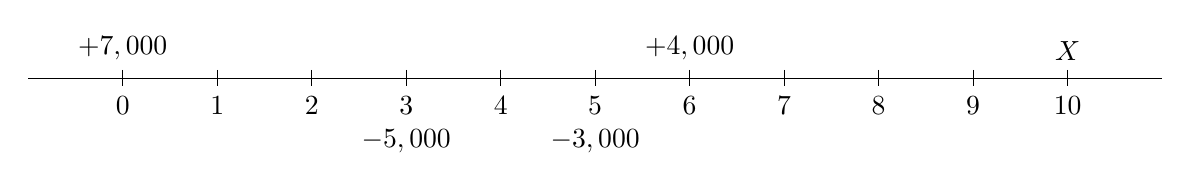
\begin{tikzpicture}
    \def\f{1.2}
    \draw (0,0) -- (\f*12,0);
    \foreach \x in {\f*1,\f*2,\f*3,\f*4,\f*5,\f*6,\f*7,\f*8,\f*9,\f*10,\f*11}
      \draw (\x cm,3pt) -- (\x cm,-3pt);
    \draw (\f*1,0) node[below=3pt, align=center] {$0$}
        node[above=3pt] {$+7,000$};
    \draw (\f*2,0) node[below=3pt, align=center] {$1$}
        node[above=3pt] {$ $};
    \draw (\f*3,0) node[below=3pt, align=center] {$2$}
        node[above=3pt] {$ $};
    \draw (\f*4,0) node[below=3pt, align=center] {$3$\\$-5,000$}
        node[above=3pt] {$ $};
    \draw (\f*5,0) node[below=3pt, align=center] {$4$}
        node[above=3pt] {$ $};
    \draw (\f*6,0) node[below=3pt, align=center] {$5$\\$-3,000$}
        node[above=3pt] {$ $};
    \draw (\f*7,0) node[below=3pt, align=center] {$6$}
        node[above=3pt] {$+4,000$};
    \draw (\f*8,0) node[below=3pt, align=center] {$7$}
        node[above=3pt] {$ $};
    \draw (\f*9,0) node[below=3pt, align=center] {$8$}
        node[above=3pt] {$ $};
    \draw (\f*10,0) node[below=3pt, align=center] {$9$}
        node[above=3pt] {$ $};
    \draw (\f*11,0) node[below=3pt, align=center] {$10$}
        node[above=3pt] {$X$};
\end{tikzpicture}
\end{center}

$i = 0.06$, how much is in the account after 10 years?

\begin{equation}\nonumber
    \begin{aligned}
        X &= 7,000(1.06)^{10} - 5,000(1.06)^7 - 3,000(1.06)^5 + 4,000(1.06)^4 \\
        X &= 6,053.01369
    \end{aligned}
\end{equation}

\subsection*{2--2}

Draw a timeline:\\

\begin{center}
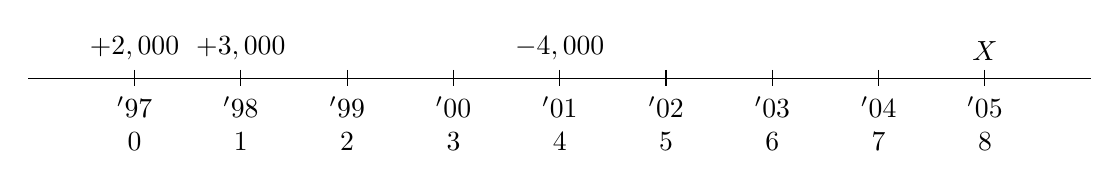
\begin{tikzpicture}
    \def\f{1.35}
    \draw (0,0) -- (\f*10,0);
    \foreach \x in {\f*1,\f*2,\f*3,\f*4,\f*5,\f*6,\f*7,\f*8,\f*9}
      \draw (\x cm,3pt) -- (\x cm,-3pt);
    \draw (\f*1,0) node[below=3pt, align=center] {$'97$\\$0$}
        node[above=3pt] {$+2,000$};
    \draw (\f*2,0) node[below=3pt, align=center] {$'98$\\$1$}
        node[above=3pt] {$+3,000$};
    \draw (\f*3,0) node[below=3pt, align=center] {$'99$\\$2$}
        node[above=3pt] {$ $};
    \draw (\f*4,0) node[below=3pt, align=center] {$'00$\\$3$}
        node[above=3pt] {$ $};
    \draw (\f*5,0) node[below=3pt, align=center] {$'01$\\$4$}
        node[above=3pt] {$-4,000$};
    \draw (\f*6,0) node[below=3pt, align=center] {$'02$\\$5$}
        node[above=3pt] {$ $};
    \draw (\f*7,0) node[below=3pt, align=center] {$'03$\\$6$}
        node[above=3pt] {$ $};
    \draw (\f*8,0) node[below=3pt, align=center] {$'04$\\$7$}
        node[above=3pt] {$ $};
    \draw (\f*9,0) node[below=3pt, align=center] {$'05$\\$8$}
        node[above=3pt] {$X$};
\end{tikzpicture}
\end{center}

$i = 0.13$, how much is owed in 2005?

\begin{equation}\nonumber
    \begin{aligned}
        X &= 2,000(1.13)^{8} + 3,000(1.13)^7 - 4,000(1.13)^4 \\
        X &= 5,852.81039
    \end{aligned}
\end{equation}


\subsection*{2--3}

Draw a timeline:\\

\begin{center}
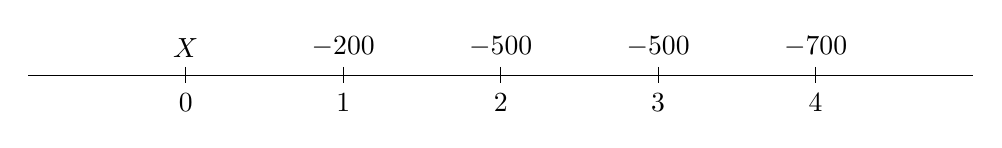
\begin{tikzpicture}
    \def\f{2}
    \draw (0,0) -- (\f*6,0);
    \foreach \x in {\f*1,\f*2,\f*3,\f*4,\f*5}
      \draw (\x cm,3pt) -- (\x cm,-3pt);
    \draw (\f*1,0) node[below=3pt, align=center] {$0$}
        node[above=3pt] {$X$};
    \draw (\f*2,0) node[below=3pt, align=center] {$1$}
        node[above=3pt] {$-200$};
    \draw (\f*3,0) node[below=3pt, align=center] {$2$}
        node[above=3pt] {$-500$};
    \draw (\f*4,0) node[below=3pt, align=center] {$3$}
        node[above=3pt] {$-500$};
    \draw (\f*5,0) node[below=3pt, align=center] {$4$}
        node[above=3pt] {$-700$};
\end{tikzpicture}
\end{center}

$i = 0.12$, at these payments, how much money can be borrowed?

\begin{equation}\nonumber
    \begin{aligned}
        X&(1.12)^4 - 200(1.12)^3 - 500(1.12)^2 - 500(1.12) - 700 = 0 \\
        X &= \frac{200}{1.12} + \frac{500}{(1.12)^2} + \frac{500}{(1.12)^3}
            + \frac{700}{(1.12)^4}  \\
        X &= 1,377.92115
    \end{aligned}
\end{equation}

\subsection*{2--4}

Draw a timeline:\\

\begin{center}
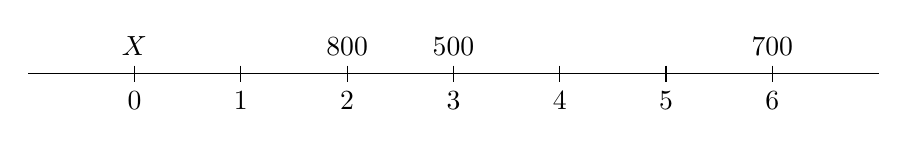
\begin{tikzpicture}
    \def\f{1.35}
    \draw (0,0) -- (\f*8,0);
    \foreach \x in {\f*1,\f*2,\f*3,\f*4,\f*5,\f*6,\f*7}
      \draw (\x cm,3pt) -- (\x cm,-3pt);
    \draw (\f*1,0) node[below=3pt, align=center] {$0$}
        node[above=3pt] {$X$};
    \draw (\f*2,0) node[below=3pt, align=center] {$1$}
        node[above=3pt] {$ $};
    \draw (\f*3,0) node[below=3pt, align=center] {$2$}
        node[above=3pt] {$800$};
    \draw (\f*4,0) node[below=3pt, align=center] {$3$}
        node[above=3pt] {$500$};
    \draw (\f*5,0) node[below=3pt, align=center] {$4$}
        node[above=3pt] {$ $};
    \draw (\f*6,0) node[below=3pt, align=center] {$5$}
        node[above=3pt] {$ $};
    \draw (\f*7,0) node[below=3pt, align=center] {$6$}
        node[above=3pt] {$700$};
\end{tikzpicture}
\end{center}

$i = 0.13$, at what time would a single payment of 2,100 be equivalent to the 
ones above?

\begin{equation}\nonumber
    \begin{aligned}
        2,100(1.13)^t &= 800(1.13)^4 + 500(1.13)^3 + 700        \\
        t &= \frac{\ln\left(800(1.13)^4 + 500(1.13)^3 + 700\right)
            - \ln(2,100)}{\ln(1.13)}                            \\
        t &= 2.13418
    \end{aligned}
\end{equation}

This result is the time from $t=6$ backwards, so to find the time from the
origin, we subtract our $t$ from 6, getting $t=3.86582$.

\subsection*{2--5}

Draw timelines:\\

\begin{center}
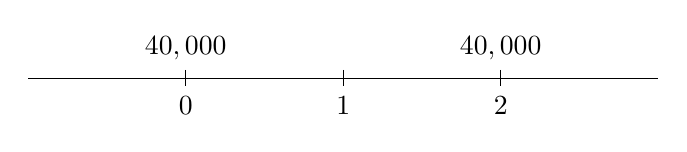
\begin{tikzpicture}
    \def\f{2}
    \draw (0,0) -- (\f*4,0);
    \foreach \x in {\f*1,\f*2,\f*3}
      \draw (\x cm,3pt) -- (\x cm,-3pt);
    \draw (\f*1,0) node[below=3pt, align=center] {$0$}
        node[above=3pt] {$40,000$};
    \draw (\f*2,0) node[below=3pt, align=center] {$1$}
        node[above=3pt] {$ $};
    \draw (\f*3,0) node[below=3pt, align=center] {$2$}
        node[above=3pt] {$40,000$};
\end{tikzpicture}
\end{center}

OR\\

\begin{center}
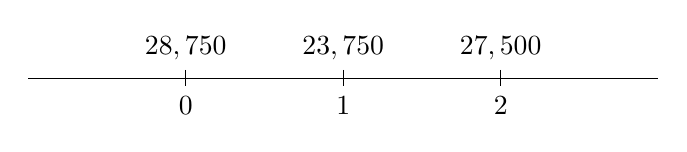
\begin{tikzpicture}
    \def\f{2}
    \draw (0,0) -- (\f*4,0);
    \foreach \x in {\f*1,\f*2,\f*3}
      \draw (\x cm,3pt) -- (\x cm,-3pt);
    \draw (\f*1,0) node[below=3pt, align=center] {$0$}
        node[above=3pt] {$28,750$};
    \draw (\f*2,0) node[below=3pt, align=center] {$1$}
        node[above=3pt] {$23,750$};
    \draw (\f*3,0) node[below=3pt, align=center] {$2$}
        node[above=3pt] {$27,500$};
\end{tikzpicture}
\end{center}

For which $i$ are these two payment plans equivalent?

\begin{equation}\nonumber
    \begin{aligned}
        40,000 + 40,000(1+i)^2 &= 28,750(1+i)^2 + 23,750(1+i) + 27,500 \\
        1+i &= c        \\
        0 &= 11,250c^2 + 23,750c + 12,500   \\
        0 &= 9c^2 - 19c + 10        \\
        c_1 = 1 &\qquad c_2 = \frac{10}{9}     \\
        i_1 = 0 &\qquad i_2 = \frac{1}{9}
    \end{aligned}
\end{equation}

\subsection*{2--6}

\begin{enumerate}[label=(\alph*)]
    \item draw a timeline\\
        \begin{center}
            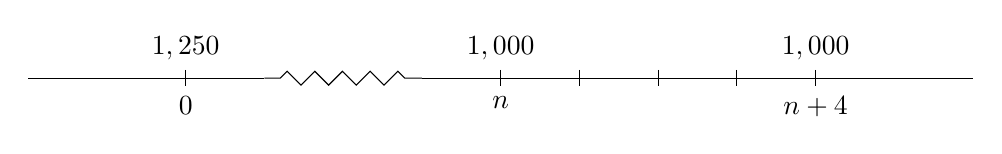
\begin{tikzpicture}[snake=zigzag, line before snake = 2mm, line
                after snake = 2mm]
                \def\f{2}
                \draw (0,0) -- (\f*1.5,0);
                \draw[snake] (\f*1.5,0) -- (\f*2.5,0);
                \draw (\f*2.5,0) -- (\f*6,0);
                \foreach \x in {\f*1,\f*3,\f*3.5,\f*4,\f*4.5,\f*5}
                  \draw (\x cm,3pt) -- (\x cm,-3pt);
                \draw (\f*1,0) node[below=3pt, align=center] {$0$}
                    node[above=3pt] {$1,250$};
                \draw (\f*3,0) node[below=3pt, align=center] {$n$}
                    node[above=3pt] {$1,000$};
                \draw (\f*5,0) node[below=3pt, align=center] {$n+4$}
                    node[above=3pt] {$1,000$};
            \end{tikzpicture}
        \end{center}

        $i = 0.08$, find $n$ if 1,250 is the present value
    
        \begin{equation}\nonumber
            \begin{aligned}
                1,000 + 1,000(1,08)^4 &= 1,250(1,08)^{n+4}          \\
                1,000(1 + 1.08^4) &= 1,250(1,08)^{n+4}                  \\
                1.08^{n+4} &= \frac{1,000(1 + 1.08^4)}{1,250}           \\
                n+4 &= \frac{\ln(1,000(1 + 1.08^4))-\ln(1,250)}{\ln(1.08)} \\
                n &= 8.26035 - 4    \\
                n &= 4.26035
            \end{aligned}
        \end{equation}
    \item draw a timeline\\
        \begin{center}
            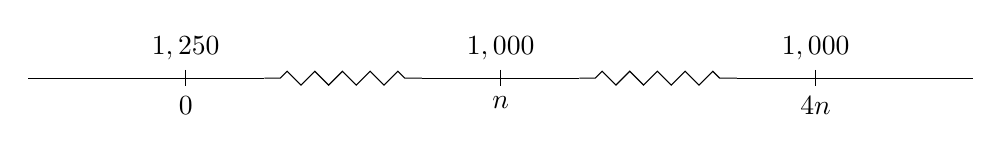
\begin{tikzpicture}[snake=zigzag, line before snake = 2mm, line
                after snake = 2mm]
                \def\f{2}
                \draw (0,0) -- (\f*1.5,0);
                \draw[snake] (\f*1.5,0) -- (\f*2.5,0);
                \draw (\f*2.5,0) -- (\f*3.5,0);
                \draw[snake] (\f*3.5,0) -- (\f*4.5,0);
                \draw (\f*4.5,0) -- (\f*6,0);
                \foreach \x in {\f*1,\f*3,\f*5}
                  \draw (\x cm,3pt) -- (\x cm,-3pt);
                \draw (\f*1,0) node[below=3pt, align=center] {$0$}
                    node[above=3pt] {$1,250$};
                \draw (\f*3,0) node[below=3pt, align=center] {$n$}
                    node[above=3pt] {$1,000$};
                \draw (\f*5,0) node[below=3pt, align=center] {$4n$}
                    node[above=3pt] {$1,000$};
            \end{tikzpicture}
        \end{center}

        if $i=0.08$ and 1,250 the present value, find $n$

        \begin{equation}\nonumber
            \begin{aligned}
                1,000 + 1,000(1.08)^{3n} &= 1,250(1.08)^{4n}            \\
                0 &= 1.25(1.08)^{4n} - (1.08)^{3n} - 1                  \\
                0 &= 1.25\left((1.08)^n\right)^4 - 
                    \left((1.08)^n\right)^3 - 1                         \\
                u &= (1.08)^n                                           \\
                0 &= 1.25u^4 - u^3 - 1                                  \\
                u_1 < 0, \quad u_2, u_3 &\text{ are complex} \quad u_4
                = 1.22995467         \\
                n &= \frac{\ln(u_4)}{\ln(1.08)}                           \\
                n &= \frac{\ln(1.22995467)}{\ln(1.08)}                  \\
                n &= 2.6893
            \end{aligned}
        \end{equation}
\end{enumerate}

\subsection*{2--7}

Draw timeline:\\

\begin{center}
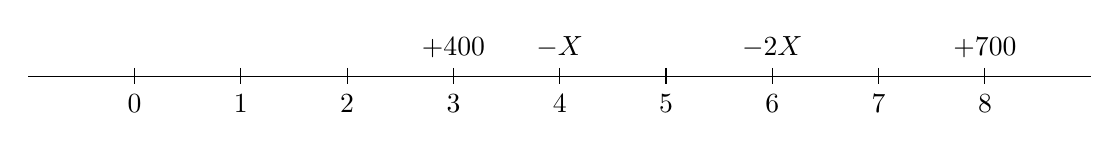
\begin{tikzpicture}
    \def\f{1.35}
    \draw (0,0) -- (\f*10,0);
    \foreach \x in {\f*1,\f*2,\f*3,\f*4,\f*5,\f*6,\f*7,\f*8,\f*9}
      \draw (\x cm,3pt) -- (\x cm,-3pt);
    \draw (\f*1,0) node[below=3pt, align=center] {$0$}
        node[above=3pt] {$ $};
    \draw (\f*2,0) node[below=3pt, align=center] {$1$}
        node[above=3pt] {$ $};
    \draw (\f*3,0) node[below=3pt, align=center] {$2$}
        node[above=3pt] {$ $};
    \draw (\f*4,0) node[below=3pt, align=center] {$3$}
        node[above=3pt] {$+400$};
    \draw (\f*5,0) node[below=3pt, align=center] {$4$}
        node[above=3pt] {$-X$};
    \draw (\f*6,0) node[below=3pt, align=center] {$5$}
        node[above=3pt] {$ $};
    \draw (\f*7,0) node[below=3pt, align=center] {$6$}
        node[above=3pt] {$-2X$};
    \draw (\f*8,0) node[below=3pt, align=center] {$7$}
        node[above=3pt] {$ $};
    \draw (\f*9,0) node[below=3pt, align=center] {$8$}
        node[above=3pt] {$+700$};
\end{tikzpicture}
\end{center}

if $i=0.14$, find $X$

\begin{equation}\nonumber
    \begin{aligned}
        400(1.14)^5 + 700 &= X(1.14)^4 + 2X(1.14)^2         \\
        X &= \frac{400(1.14)^5 + 700}{(1.14)^4 + 2(1.14)^2} \\
        X &= 342.843
    \end{aligned}
\end{equation}

\subsection*{2--8}

At what point are 1,000 at $i=0.12$ equal to twice 1,000 at $i=0.09$?

\begin{equation}\nonumber
    \begin{aligned}
        1,000(1.12)^t &= 2 \cdot 1000(1.08)^t               \\
        t\ln(1.12) &= \ln(2) + t\ln(1.08)                   \\
        t &= \frac{\ln(2)}{\ln(1.12) - \ln(1.08)}           \\
        t &= 19.05945
    \end{aligned}
\end{equation}

\subsection*{2--9}

Draw a timeline:\\

\begin{center}
    \begin{tikzpicture}[snake=zigzag, line before snake = 2mm, line
        after snake = 2mm]
        \def\f{2}
        \draw (0,0) -- (\f*1.5,0);
        \draw[snake] (\f*1.5,0) -- (\f*2.5,0);
        \draw (\f*2.5,0) -- (\f*4.5,0);
        \draw[snake] (\f*4.5,0) -- (\f*5.5,0);
        \draw (\f*5.5,0) -- (\f*7,0);
        \foreach \x in {\f*1,\f*3,\f*4,\f*6}
          \draw (\x cm,3pt) -- (\x cm,-3pt);
        \draw (\f*1,0) node[below=3pt, align=center] {$0$}
            node[above=3pt] {$ $};
        \draw (\f*3,0) node[below=3pt, align=center] {$8$}
            node[above=3pt] {$B=3A$};
        \draw (\f*4,0) node[below=3pt, align=center] {$10$}
            node[above=3pt,align=center] {$A+B=$\\$50,000$};
        \draw (\f*6,0) node[below=3pt, align=center] {$15$}
            node[above=3pt] {$A$};
    \end{tikzpicture}
\end{center}

$i_B=0.08$, $i_A=0.09$\\
At $t=8$ $B=3A$ and thus $B(1.08)^8=3A(1.09)^8$ and 
$B_8 = 3A(1.09)^8(1.08)^{-8}$. \\
This means that at $t=10$, $B_{10} = B_8(1.08)^2$ or 
$B_{10} = 3A(1.09)^8(1.08)^{-6}$.

\begin{equation}\nonumber
    \begin{aligned}
        A_{10} + B_{10} &= 52,000  \\
        A(1.09)^{10} + 3A(1.09)^8(1.08)^{-6} &= 52,000 \\
        A_8 &= \frac{52,000}{(1.09)^{2} + 3(1.08)^{-6}} \\
        A_{15} &= A_8 \cdot (1.09)^7                        \\
        A_{15} &= \frac{52,000}{(1.09)^{2} + 3(1.08)^{-6}} * (1.09)^7   \\
        A_{15} &= 30,876.94409
    \end{aligned}
\end{equation}

\subsection*{2--10}

Timeline for this problem:\\

\begin{center}
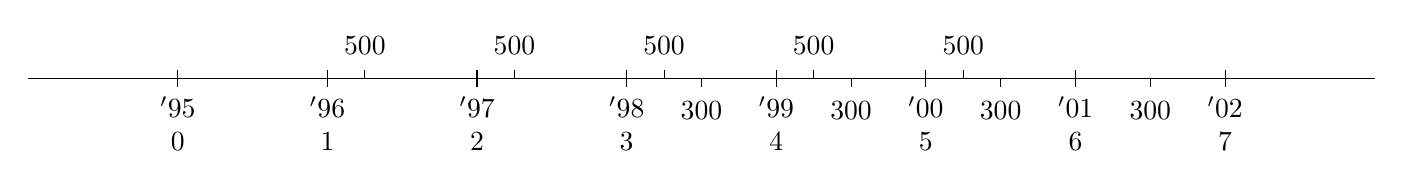
\begin{tikzpicture}
    \def\f{1.9}
    \draw (0,0) -- (\f*9,0);
    \foreach \x in {\f*1,\f*2,\f*3,\f*4,\f*5,\f*6,\f*7,\f*8}
      \draw (\x cm,3pt) -- (\x cm,-3pt);

    \foreach \y in {\f*2.25,\f*3.25,\f*4.25,\f*5.25,\f*6.25}
      \draw (\y cm,3pt) -- (\y cm,0pt);
      
    \foreach \y in {\f*4.5,\f*5.5,\f*6.5,\f*7.5}
      \draw (\y cm,0pt) -- (\y cm,-3pt);

    \draw (\f*1,0) node[below=3pt, align=center] {$'95$\\$0$}
        node[above=3pt] {$ $};

    \draw (\f*2,0) node[below=3pt, align=center] {$'96$\\$1$}
        node[above=3pt] {$ $};
    \draw (\f*2.25,0) node[below=3pt, align=center] {$ $}
        node[above=5pt] {$500$};

    \draw (\f*3,0) node[below=3pt, align=center] {$'97$\\$2$}
        node[above=3pt] {$ $};
    \draw (\f*3.25,0) node[below=3pt, align=center] {$ $}
        node[above=5pt] {$500$};

    \draw (\f*4,0) node[below=3pt, align=center] {$'98$\\$3$}
        node[above=3pt] {$ $};
    \draw (\f*4.25,0) node[below=3pt, align=center] {$ $}
        node[above=5pt] {$500$};
    \draw (\f*4.5,0) node[below=5pt, align=center] {$300$}
        node[above=3pt] {$ $};
        
    \draw (\f*5,0) node[below=3pt, align=center] {$'99$\\$4$}
        node[above=3pt] {$ $};
    \draw (\f*5.25,0) node[below=3pt, align=center] {$ $}
        node[above=5pt] {$500$};
    \draw (\f*5.5,0) node[below=5pt, align=center] {$300$}
        node[above=3pt] {$ $};

    \draw (\f*6,0) node[below=3pt, align=center] {$'00$\\$5$}
        node[above=3pt] {$ $};
    \draw (\f*6.25,0) node[below=3pt, align=center] {$ $}
        node[above=5pt] {$500$};
    \draw (\f*6.5,0) node[below=5pt, align=center] {$300$}
        node[above=3pt] {$ $};

    \draw (\f*7,0) node[below=3pt, align=center] {$'01$\\$6$}
        node[above=3pt] {$ $};
    \draw (\f*7.5,0) node[below=5pt, align=center] {$300$}
        node[above=3pt] {$ $};

    \draw (\f*8,0) node[below=3pt, align=center] {$'02$\\$7$}
        node[above=3pt] {$ $};
\end{tikzpicture}
\end{center}

Find the total value of the payments on March 15, 2002

\begin{equation}\nonumber
    V = \sum_{j=2}^6{500\left(1+\frac{17}{400}\right)^{4j}}
        + \sum_{j=1}^4{300\left(1+\frac{17}{400}\right)^{4j-1}} 
\end{equation}

\begin{enumerate}[label=(\alph*)]
    \item Value on March 15, 2005
        \begin{equation}\nonumber
            \begin{aligned}
                X &= V \cdot \left(1 + \frac{17}{400}\right)^3      \\
                X &= 7,678.792345
            \end{aligned}
        \end{equation}
    \item Value on March 15, 1999
        \begin{equation}\nonumber
            \begin{aligned}
                X &= V \cdot \left(1 + \frac{17}{400}\right)^{-3}   \\
                X &= 5,981.864088
            \end{aligned}
        \end{equation}
    \item Value on March 15, 1995
        \begin{equation}\nonumber
            \begin{aligned}
                X &= V \cdot \left(1 + \frac{17}{400}\right)^{-7}   \\
                X &= 5,064.449988
            \end{aligned}
        \end{equation}
\end{enumerate}

\end{document}
